%% Seção 5: As Dinâmicas de Poder e o Contexto Sociocultural

\chapter{As Dinâmicas de Poder e o Contexto Sociocultural Afetam a Linguagem e o Comportamento do Paciente}

\epigrafe{O poder está em toda parte; não porque englobe tudo, e sim porque provém de todos os lugares.}{Michel Foucault, \textit{História da Sexualidade}}

\textbf{5.} As dinâmicas de poder e o contexto sociocultural afetam profundamente a maneira como a linguagem se organiza, influenciando a subjetividade e a construção do self.

\section{Subjetividade e relações de poder}

\textbf{5.1} A subjetividade do paciente é uma construção permeada pelas relações de poder internalizadas.

\begin{tese}
Se as relações de poder moldam a subjetividade (conforme Foucault), então a linguagem que o paciente utiliza reflete essas dinâmicas de poder internalizadas.
\end{tese}

\begin{hipotese}[title=Hipótese 5.1.1 (Condicional)]
Se o paciente internaliza relações de poder, então sua linguagem reproduz estruturas de dominação e submissão.
\end{hipotese}

\begin{referencia}[title=Referência a Foucault]
Michel Foucault argumenta que o poder se exerce através de discursos que produzem e regulam as práticas sociais, influenciando a subjetividade dos indivíduos.
\end{referencia}

\begin{aforismo}
As palavras carregam em si as marcas invisíveis das forças que as moldam.
\end{aforismo}

\section{Reprodução de hierarquias através da linguagem}

\textbf{5.11} O paciente reproduz, através de sua linguagem, as hierarquias de poder que moldaram sua vida.

\begin{tese}
Se a linguagem é um instrumento de poder (conforme Marx e Engels), então o discurso do paciente reflete as ideologias dominantes que o influenciam.
\end{tese}

\begin{referencia}[title=Referência a Marx e Engels]
A ideologia dominante é a ideologia da classe dominante; a linguagem pode ser um veículo de reprodução das relações de classe.
\end{referencia}

\begin{aforismo}
A língua do oprimido muitas vezes fala com a voz do opressor.
\end{aforismo}

\section{Desconstrução e reestruturação da subjetividade}

\textbf{5.2} A desconstrução dessas relações através da fala pode gerar uma reestruturação da subjetividade, promovendo a autonomia.

\begin{tese}
Se ao tomar consciência das dinâmicas de poder que o afetam, o paciente pode ressignificar sua linguagem (conforme Hegel), então ele pode reestruturar sua subjetividade.
\end{tese}

\begin{referencia}[title=Referência a Hegel]
A dialética permite a superação das contradições através da síntese, levando ao autoconhecimento e à liberdade.
\end{referencia}

\begin{aforismo}
Ao reconhecer as correntes que o prendem, o espírito encontra o caminho para a liberdade.
\end{aforismo}

\section{Nuances e reestruturação da percepção}

\textbf{5.21} A linguagem revela essas dinâmicas, e o terapeuta, ao perceber as nuances, pode guiar o paciente na reestruturação de sua percepção de si, promovendo a emancipação.

\begin{tese}
Se o terapeuta compreende as influências socioculturais e de poder na linguagem do paciente, então pode facilitar o processo de emancipação e autonomia (conforme Hannah Arendt).
\end{tese}

\begin{referencia}[title=Referência a Hannah Arendt]
A ação e o discurso são fundamentais para a manifestação da liberdade e da identidade no espaço público.
\end{referencia}

\begin{aforismo}
É na palavra que se ergue contra a opressão que a liberdade encontra voz.
\end{aforismo}

\section{Contexto sociocultural e gramática emocional}

\textbf{5.3} O contexto sociocultural é um plano de fundo que define a gramática emocional do paciente.

\begin{tese}
Se o contexto sociocultural influencia a expressão das emoções (conforme Brecht), então a compreensão desse contexto é essencial para interpretar corretamente o discurso e suas lacunas.
\end{tese}

\begin{referencia}[title=Referência a Bertolt Brecht]
A arte e a expressão humana são influenciadas pelas condições materiais e sociais; a compreensão crítica dessas condições é essencial para a transformação.
\end{referencia}

\begin{aforismo}
As emoções dançam ao som da música que a sociedade toca.
\end{aforismo}

\section{Valores e normas culturais na linguagem}

\textbf{5.31} O discurso do paciente é sempre ancorado em um sistema de valores e normas herdadas do seu meio cultural, que podem limitar ou potencializar sua autonomia.

\begin{tese}
Se os valores e normas culturais influenciam a subjetividade (conforme Marx), então a conscientização dessas influências é necessária para a transformação pessoal.
\end{tese}

\begin{aforismo}
Conhecer as raízes de suas palavras é desvendar as origens de si mesmo.
\end{aforismo}

\section{Interpretação do discurso através do contexto}

\textbf{5.32} O terapeuta deve entender o contexto sociocultural para interpretar corretamente o discurso e suas lacunas, auxiliando o paciente na construção de uma identidade autêntica.

\begin{referencia}[title=Referência a Arendt]
A autenticidade surge quando o indivíduo age e fala em consonância com sua singularidade, apesar das pressões sociais.
\end{referencia}

\begin{aforismo}
Ao compreender o mundo que o cerca, o indivíduo encontra o caminho para ser verdadeiramente ele mesmo.
\end{aforismo}

\section{O triângulo de poder, cultura e subjetividade}

\textbf{5.4} O poder, a cultura e a subjetividade formam um triângulo que define a maneira como a linguagem do paciente é estruturada, influenciando sua cognição e emoção.

\begin{tese}
Se a linguagem está no centro das interações entre poder, cultura e subjetividade, então a transformação da linguagem pode levar à transformação do self (conforme Paulo Freire).
\end{tese}

\begin{referencia}[title=Referência a Paulo Freire]
A conscientização é o processo pelo qual o indivíduo percebe as contradições sociais e atua para transformar a realidade.
\end{referencia}

\begin{aforismo}
Na palavra conscientizada, o oprimido reencontra sua humanidade.
\end{aforismo}

%% DIAGRAMA DO TRIÂNGULO
\section*{Diagrama Representativo: O Triângulo do Poder, Cultura e Subjetividade}

\begin{center}
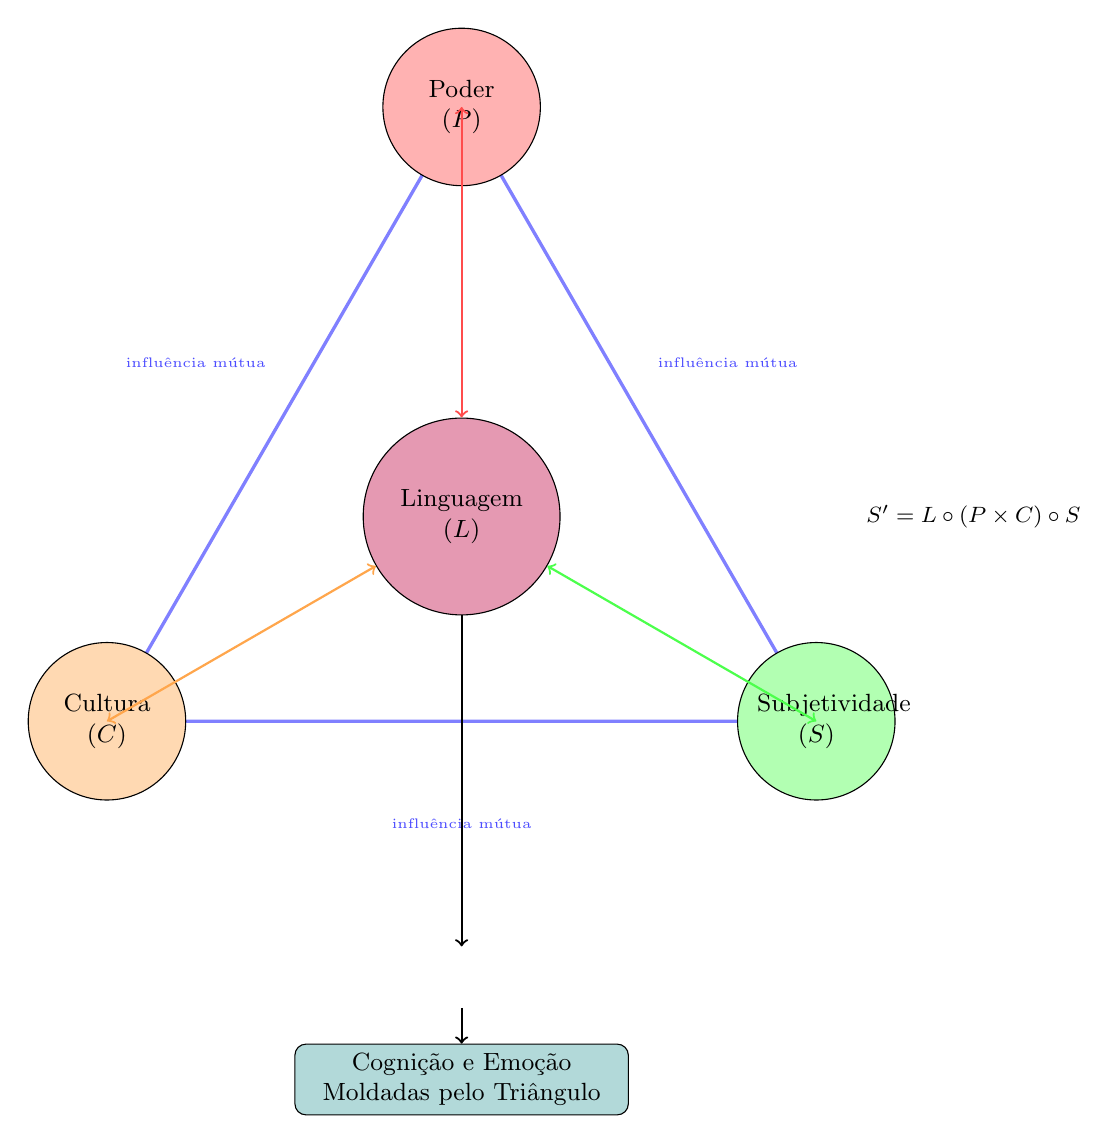
\begin{tikzpicture}[scale=1.3, every node/.style={font=\small}]
    % Vértices do triângulo
    \coordinate (P) at (90:4);      % Poder
    \coordinate (C) at (210:4);     % Cultura
    \coordinate (S) at (330:4);     % Subjetividade

    % Triângulo
    \draw[very thick, blue!50] (P) -- (C) -- (S) -- cycle;

    % Nós nos vértices
    \node[draw, circle, fill=red!30, minimum size=2cm, text width=1.5cm, align=center] at (P) {Poder\\$(P)$};
    \node[draw, circle, fill=orange!30, minimum size=2cm, text width=1.5cm, align=center] at (C) {Cultura\\$(C)$};
    \node[draw, circle, fill=green!30, minimum size=2cm, text width=1.5cm, align=center] at (S) {Subjetividade\\$(S)$};

    % Centro - Linguagem
    \node[draw, circle, fill=purple!40, minimum size=2.5cm, text width=2cm, align=center] (L) at (0,0) {Linguagem\\$(L)$};

    % Setas bidirecionais dos vértices para o centro
    \draw[thick, <->, red!70] (P) -- (L);
    \draw[thick, <->, orange!70] (C) -- (L);
    \draw[thick, <->, green!70] (S) -- (L);

    % Labels nas arestas
    \node[font=\tiny, blue!70] at (150:3) {influência mútua};
    \node[font=\tiny, blue!70] at (270:3) {influência mútua};
    \node[font=\tiny, blue!70] at (30:3) {influência mútua};

    % Resultado
    \node[draw, rounded corners, fill=teal!30, text width=4cm, align=center] (result) at (0,-5.5) {Cognição e Emoção\\Moldadas pelo Triângulo};
    \draw[thick, ->] (L) -- (0,-4.2);
    \draw[thick, ->] (0,-4.8) -- (result);

    % Fórmula
    \node[font=\footnotesize] at (5,0) {$S' = L \circ (P \times C) \circ S$};
\end{tikzpicture}
\end{center}

\begin{sintese}[title=Síntese Final da Seção 5]
As dinâmicas de poder e o contexto sociocultural afetam profundamente a maneira como a linguagem do paciente é estruturada, influenciando sua subjetividade, cognição e emoção. Conforme Foucault, as relações de poder permeiam os discursos e moldam a subjetividade. Marx e Engels destacam que a linguagem pode ser um veículo de reprodução das ideologias dominantes, enquanto Hegel propõe que a consciência crítica permite a superação das contradições e a busca pela liberdade.

A compreensão dessas influências é essencial para o terapeuta, que, ao perceber as nuances e lacunas no discurso do paciente, pode guiá-lo na reestruturação de sua percepção de si, promovendo a emancipação e a construção de uma identidade autêntica. O poder, a cultura e a subjetividade formam um triângulo dinâmico, com a linguagem no centro dessa interação. Ao transformar sua linguagem de forma crítica e consciente, o paciente pode redefinir sua posição em relação às estruturas de poder e cultura, avançando em direção à autonomia e à autenticidade do ser.
\end{sintese}

\nextpage
